\documentclass[a4paper,16pt,UTF8]{article}
    % 宏包的使用
    \usepackage{ctex}
    \usepackage{verbatim}
    \usepackage{graphicx}
    \usepackage{upgreek}
    \usepackage{longtable}
    \usepackage{geometry}
    \usepackage{graphics}
    \usepackage{booktabs}

    \graphicspath{{pic/}}

\begin{document}

\title{\Huge 大地测量实验报告}
\author{1551127 任家平}
\date{\today}
\maketitle

\newpage

\section{\LARGE 概述}

\subsection{\Large 实习目的与意义}
将所学的控制测量、GPS测量的基本概念、基本理论、基本方法系统地应用到实际作业中。通过实践,进一步加深和巩固学生所学的理论知识,同时培养学生独立的实际工作能力,以及分析问题和解决问题的能力,更要培养学生的吃苦耐劳、团结协作、认真负责、一丝不苟的敬业精神。

\subsection{\Large 实习任务}
\begin{itemize}
    \item 掌握平面和高程控制网的设计和布设
    \item 熟练掌握GPS接收机、精密经纬仪、测距仪、全站仪和水准仪的操作
    \item 从事平面和高程控制网野外测量工作
    \item 能独立进行GPS基线、网平差处理,以及常规平面和高程控制网的数据处理
\end{itemize}

\subsection{\Large 测区概况}
\begin{center}
    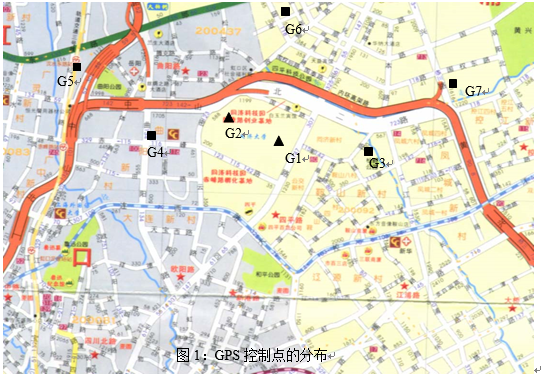
\includegraphics[height = 9 cm]{cequ.jpg}
\end{center}

实习区域位于以同济大学为中心、向四周各扩展1 ~ 2公里的区域内。测区位于上海市中心城区,道路密布、交通发达,有55路、123路、142路等公共汽车可以直达。测区的纬度约$31^{\circ}17'$、经度约$121^{\circ}30'$,属于海洋性温带气候,四季分明,雨量充沛。




\section{\LARGE 高程控制测量}

\subsection{\Large 概述}

本次高程控制测量为在同济大学四平路校区的精密水准测量。水准路线是长度大致为2.5km的闭合环,起点从北楼高程控制点开始,经过外国语学院、文远楼与三好坞到达北门高程待测点,从该待测点出发,向西经过西北一西北三宿舍楼,向南经过宁静楼,致远楼和南门停车场到达西南高程待测控制点,再经西南高程控制点出发,向东经过快递中心,西南九西南八,西南七宿舍楼,医学院大楼,一二九操场,向北经过南楼,到达北楼高程已知控制点。

水准路线如下图所示:

\begin{center}
    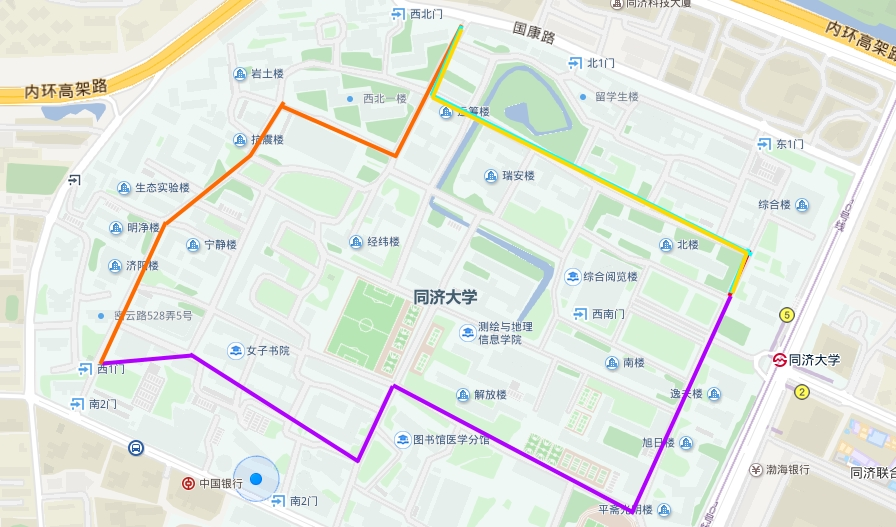
\includegraphics[scale = 0.45]{uvvp.jpg}

    黄色表示从北楼的已知高程控制点到北门待测高程控制点线路

    橘色表示从北门待测高程控制点到西南门待测高程控制点线路

    紫色表示从西南门待测高程控制点到北楼已知高程控制点线路
\end{center}


\subsection{\Large 限差要求}

按二等精密水准的要求,一个测站观测数据的各项限差:
\begin{enumerate}
    \item 视线长度$\leq$ 50米,前后视距差$\leq$ 1.0米,前后视距累积差$\leq$ 3.0米
    \item 视线高度$\geq$ 0.3米,基辅差$\leq$ 0.5毫米,高差之差$\leq$ 0.7毫米
    \item 临时点高程检查$\leq$ 1.0毫米,上下丝平均值与中丝之差$\leq$ 3.0毫米
    \item 往返测与附合水准路线高差的限差:$40 \sqrt{k}$ (mm)。其中,k为水准路线的长度,单位为公里。
\end{enumerate}


\subsection{\Large 直接平差}
根据实习要求,每个小组成员负责一条边往返的水准测量。本人负责北门至西南门高程控制点的往测和西南门到北门高程控制点的返测,即第二次往返测。测量的记录手稿详见附录,最终的计算表格如下:

\begin{center}
    \setlength\tabcolsep{4pt}
    \begin{longtable}{|c|c|c|c|c|c|c|c|c|}
        \caption{第二次往测} \\ \hline
        路线    & 长度    & 权     & 高差    & 改正数乘积 & 改正数   & 平差值   & 2.698000  &  \\ \hline
        北楼 至 北门 & 641.01  & 0.001560  & 0.463385  & 0.195572  & -0.000291  & 0.463094  & 3.161094  & 北门 \\ \hline
        北门 至TGP4 & 419.15  & 0.002386  & 0.271095  & 0.299090  & -0.000446  & 0.270649  & 3.431743  & TGP4 \\ \hline
        TGP4 至 西南 & 317.47  & 0.003150  & -0.101320  & 0.394883  & -0.000588  & -0.101908  & 3.329835  & 西南 \\ \hline
        西南 至 北楼 & 1134.96  & 0.000881  & -0.631670  & 0.110456  & -0.000165  & -0.631835  & 2.698000  & 北楼 \\ \hline
        求和    & 2512.59  & 0.007977  & 0.001490  & 1.000000  &       & 0.000000  &       &  \\ \hline
    \end{longtable}

    \setlength\tabcolsep{4pt}
    \begin{longtable}{|c|c|c|c|c|c|c|c|c|}
        \caption{第二次返测} \\ \hline
        路线    & 长度    & 权     & 高差    & 改正数乘积 & 改正数   & 平差值   & 2.698000  &  \\ \hline
        北楼 至 西南 & 1143.76  & 0.000874  & 0.633170  & 0.114954  & 0.000280  & 0.633450  & 3.331450  & 西南 \\ \hline
        西南至TGP4 & 369.62  & 0.002705  & 0.100705  & 0.355717  & 0.000866  & 0.101571  & 3.433021  & TGP4 \\ \hline
        TGP4 至 北门 & 413.18  & 0.002420  & -0.269250  & 0.318215  & 0.000775  & -0.268475  & 3.164546  & 北门 \\ \hline
        北门 至 北楼 & 622.79  & 0.001606  & -0.467060  & 0.211114  & 0.000514  & -0.466546  & 2.698000  & 北楼 \\ \hline
        求和    & 2549.35  & 0.007606  & -0.002435  & 1.000000  &       & 0.000000  &       &  \\ \hline
    \end{longtable}
   

\end{center}


根据精密二等水准控制测量的限差要求,视线长度皆小于50m,前后视距差小于1m,前后视距差的累积小于3m(可见于附件)。
$k = 2.5km$,则闭合差的限差为$4 \times \sqrt{k} = 6.32 mm$
可在表格中容易得到往返的闭合差为1.49mm和2.43mm,闭合差并没有超限。因此数据合格。

由北楼已知高程控制点的高程,经二等水准精密测量,直接平差后,可得北门待测控制点的高程为$3.1628m$,TGP-4高程为$3.4318m$,北门高程为$3.3297m$。如下表所示:

\begin{center}
    \begin{longtable}{|c|c|}
        \caption{待测点高程} \\ \hline
        点位 & 高程(m)  \\ \hline
        北门 & 3.1628   \\ \hline
        TGP-4 & 3.4318 \\ \hline
        西南门 & 3.3297 \\ \hline
    \end{longtable}
\end{center}

\subsection{\Large 间接平差}
通过间接平差求取各个高程待测点的高程与其测量精度,其思路为将其2个往测2个返测共组成的4个闭合环所得的16段高程数据统一进行间接平差。平差结果如下:

\begin{center}
    \begin{longtable}{|c|c|c|c|}
        \caption{间接平差结果} \\ \hline
        序号    & 高差观测值(mm) & 高差改正值(mm) & 高差平差值 \\ \hline
        北门    & 463.355  & 0.5463 & 463.901 \\ \hline
        TGP4    & 270.900  & -0.4691 & 270.431 \\ \hline
        西南    & -101.730 & 0.1462 & -101.584 \\ \hline
        北楼    & -632.750 & 0.0016 & -632.748 \\ \hline
        北门    & -462.810 & -1.0913 & -463.901 \\ \hline
        TGP4   & -271.190 & 0.7591 & -270.431 \\ \hline
        西南    & 102.000  & -0.4162 & 101.584 \\ \hline
        北楼    & 631.615  & 1.1334 & 632.748 \\ \hline
        北门    & 463.385  & 0.5163 & 463.901 \\ \hline
        TGP4    & 271.095  & -0.6641 & 270.431 \\ \hline
        西南    & -101.320 & -0.2638 & -101.584 \\ \hline
        北楼    & -631.670 & -1.0784 & -632.748 \\ \hline
        北门    & -467.060 & 3.1587 & -463.901 \\ \hline
        TGP4    & -269.250 & -1.1809 & -270.431 \\ \hline
        西南    & 100.705  & 0.8788 & 101.584 \\ \hline
        北楼    & 633.170  & -0.4216 & 632.748 \\ \hline 
    \end{longtable}

    \begin{longtable}{|c|c|}
        \caption{待测点高程} \\ \hline
        点位 & 高程(m)  \\ \hline
        北门 & 3.15290   \\ \hline
        TGP-4 & 3.43233 \\ \hline
        西南门 & 3.33075 \\ \hline
    \end{longtable}

    \begin{flushleft}
        其精度评定为:

        单位权中误差:
    \end{flushleft}
    
    $\hat{\sigma}_{0}$ = $\sqrt{\frac{V^{T}PV}{n-t}}$ = $1.53mm$ 

    \begin{flushleft}
        高程中误差:
    \end{flushleft}

    $\sigma_{\hat{x}\hat{x}}$ = $\hat{\sigma}_{0} \times \sqrt{(A^{T}PA)^{-1}}$

    \begin{longtable}{|c|c|}
        \hline
        点号 & 精度$\sigma_{\hat{x}_{i}}$ \\ \hline
        北门 & 0.52274 \\ \hline
        TGP4 & 0.59933 \\ \hline
        西南 & 0.60610 \\ \hline
        \caption{精度评定} \\ 
    \end{longtable}

    
    

\end{center}

\newpage
\section{\LARGE GPS测量}

\subsection{\Large 坐标系与高程系}
\begin{itemize}
    \item 中央子午线选取经度$121^{\circ} 30′ E$,纬度原点选取$31^{\circ} 17′ N$。
    \item 投影方法采用横轴墨卡托投影。
    \item GPS 测量采用WGS-84 坐标系,已知点坐标系为上海市独立坐标系。
    \item 高程系统采用1985 国家高程基准。
\end{itemize}

\subsection{\Large 已知点坐标}
GPS网以同济大学GPS长期跟踪站G1、第三食堂前草坪上的控制点G2(即测量学任务书中的239点)为起始点,向北、东、西方向扩展了GPS控制点G3、G4、G5、G6、G7,各控制点的位置如上图所示。

两个已知点属于上海市城建坐标系,其起始点是上海国际饭店,投影面高程为5米;坐标原点的中央子午线经度采用$121.46633^{\circ}$,x坐标的加常数为-3457.13123 km,y坐标的加常数为-0.00002 km。G1点的已知x坐标为:5391.88米、y坐标3091.41米;G2点的已知x坐标为:5703.239米、y坐标2623.323米、高程为3.494米。水准点高程H=2.698米。

\subsection{\Large 控制点的选择}
关于控制点的选择所需要的遵守:
\begin{enumerate}
    \item 点位应设在易于安装接收设备,视野开阔的较高点上。视场内障碍物的高度角应小于$15^{\circ}$,减少GPS 信号的遮挡或被障碍物吸收。
    \item 点位附近不应有大面积水域和强烈干扰卫星信号接收物体,以减弱多路径效应的影响。
    \item 点位应选择在交通便利,地面基础稳固的地方,便于点的保存。   
\end{enumerate}

根据以上原则,在测绘学院和岩土楼上分别设立两个GPS带测点,分别命名为测绘1、测绘2、岩土1和岩土2。在和平公园和曲阳公园分别设立6个GPS待测点,分别命名为和平1-6,曲阳1-6.根据已知点TGP-4和测绘馆基站TJBS,可通过GPS测量分别确定各个待测点的坐标。其中TJBS为基站,不需要在该点放置接收机。

架站的顺序分别为:
\begin{itemize}
    \item 测绘1、岩土1、TPG-4
    \item 测绘2、岩土2、TGP-4
    \item 测绘1、岩土1、曲阳1、曲阳2、曲阳3
    \item 测绘2、岩土2、曲阳4、曲阳5、曲阳6
    \item 测绘1、岩土1、和平1、和平2、和平3
    \item 测绘2、岩土2、和平4、和平5、和平6
\end{itemize}

\subsection{\Large GPS网型的设计}
根据网形闭合独立环不超过五条基线边;相邻点最小距离应为平均距离的1/2—1/3;最大距离应为平均距离的2—3倍等设计原则,结合同济大学校园地形与控制点的分布情况,确定大致网形如图所示:

\begin{center}
    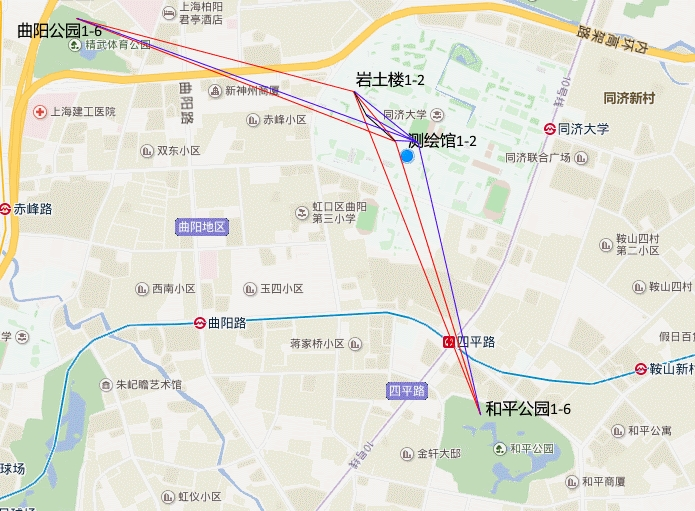
\includegraphics[scale = 0.8]{dadi.jpg}
\end{center}


\subsection{\Large 技术要求}
本次实习的GPS控制网按照城市四等的精度要求进行施测。其技术要求如下表所示:

\begin{center}
    \begin{longtable}{|c|c|c|c|c|}
        \caption{GPS网的主要要求} \\ \hline
        等级 & 平均距离(km) & a(mm) & b($10^{-6}$) & 最弱边相对中误差 \\ \hline
        二等    & 9 & $\leq$ 10    & $\leq$2     & 1/120000 \\ \hline
        三等    & 5 & $\leq$ 10    & $\leq$5     & 1/80000 \\ \hline
        四等    & 2 & $\leq$ 10    & $\leq$10    & 1/45000 \\ \hline
        一级    & 1 & $\leq$ 10    & $\leq$10    & 1/20000 \\ \hline
        二级    & <1& $\leq$ 15    & $\leq$20    & 1/10000 \\ \hline
    \end{longtable}
\end{center}

各等级城市GPS控制网的野外作业技术要求如表2 所示,本次实习野外作业采用静态测量的模式,观测时间为60分钟

\begin{center}
    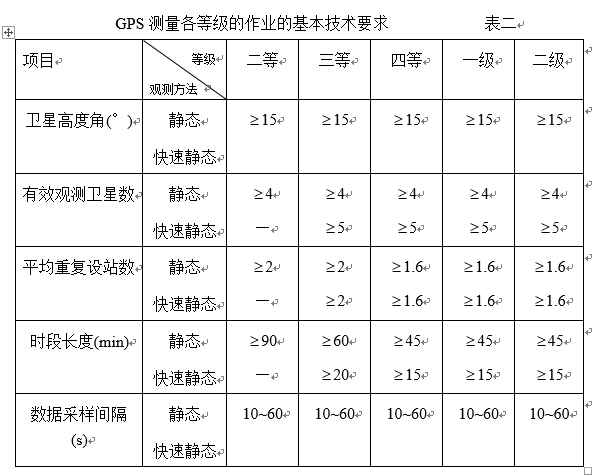
\includegraphics[scale = 1]{tab1.png}
\end{center}

各等级城市GPS控制网独立基线闭合环的限差要求如表3所示,考虑到GPS测量的精度较高,本次实习按三等的闭合差限差要求

\begin{longtable}{|c|c|c|c|c|c|}
    \caption{同步环坐标分量及环线全长相对闭合差的规定($10^{-6}$)}
    \\ \hline
          & 二等 & 三等 & 四等 & 一级 & 二级 \\ \hline
    坐标分量和相对闭合差 & 2 & 3 & 6 & 9 & 9 \\ \hline
    环线全长相对闭合差 & 3 & 5 & 10 & 15 & 15 \\ \hline
\end{longtable}

本次实验使用华测CGO软件进行基线处理与平差计算,本人负责和平公2、曲阳2的测点

\subsection{\Large GPS基线的解算}

\begin{center}
    \begin{longtable}{|c|c|c|c|c|c|}
        \caption{基线表格} \\ \hline
        X中误差  & Y分量   & Y中误差  & Z分量   & Z中误差  & 斜距 \\ \hline
        0.001792  & -473.320206  & 0.003282  & -205.435769  & 0.001705  & 1187.942690  \\ \hline
        0.002049  & -522.454665  & 0.003747  & -492.728656  & 0.001799  & 1628.358120  \\\hline
        0.001040  & -49.136313  & 0.001796  & -287.282678  & 0.000810  & 488.004761  \\ \hline
        0.001500  & -484.206195  & 0.002289  & 1013.345493  & 0.001113  & 1175.896438  \\ \hline
        0.001656  & -435.039784  & 0.002476  & 1300.624023  & 0.001337  & 1558.295143  \\ \hline
        0.000375  & 49.144977  & 0.000412  & 287.295988  & 0.000326  & 488.011272  \\ \hline
        0.000407  & 3.947848  & 0.001138  & 103.572073  & 0.000829  & 122.252088  \\ \hline
        0.000517  & -45.208552  & 0.003607  & -183.717390  & 0.001738  & 377.421152  \\ \hline
        0.000311  & -49.157591  & 0.000645  & -287.290395  & 0.000627  & 488.005997  \\ \hline
        0.002850  & -576.349129  & 0.004589  & -570.938396  & 0.002123  & 1816.095003  \\ \hline
        0.001415  & -103.040945  & 0.002640  & -365.491544  & 0.001072  & 672.304732  \\ \hline
        0.000603  & -53.899548  & 0.001177  & -78.198728  & 0.000626  & 188.978726  \\ \hline
        0.002324  & -538.095091  & 0.003030  & 935.150455  & 0.001958  & 1094.667422  \\ \hline
        0.000472  & -53.906641  & 0.000480  & -78.195552  & 0.000390  & 188.971867  \\ \hline
        0.000498  & -103.051202  & 0.000530  & -365.490912  & 0.000420  & 672.297409  \\ \hline
        0.000539  & -99.117874  & 0.001501  & -261.920661  & 0.001093  & 564.337060  \\ \hline
        0.000370  & -103.062455  & 0.000741  & -365.493802  & 0.000733  & 672.299216  \\ \hline
        0.000431  & -53.904425  & 0.000794  & -78.195030  & 0.000603  & 188.972528  \\ \hline
    \end{longtable}
\end{center}

\subsection{\Large 自由网平差}

\begin{center}
        
    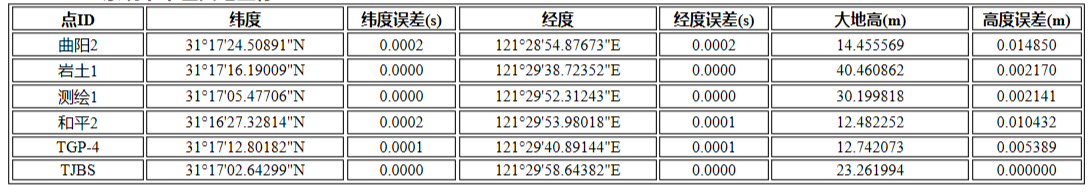
\includegraphics[scale = 0.55]{cgo2.png}
    WGS84系统下平差大地坐标
    
    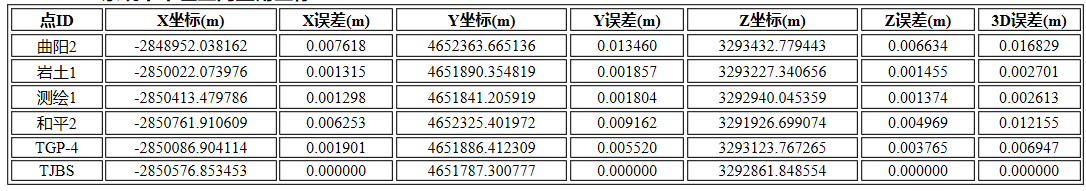
\includegraphics[scale = 0.55]{cgo3.png}
    WGS84系统下平差空间直角坐标

    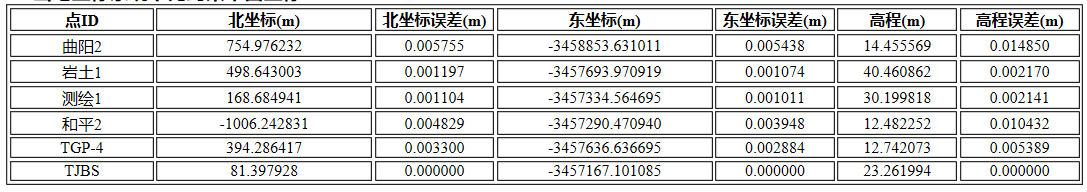
\includegraphics[scale = 0.55]{cgo4.png}
    当地坐标系统下无约束平面坐标
\end{center}

\begin{center}
    \begin{longtable}{|c|c|c|c|}
    \caption{自由网坐标变换量} \\ \hline
    点ID   & 北坐标   & 东坐标   & 大地高 \\ \hline
    曲阳2   & -0.015444  & -0.000777  & 0.010959  \\ \hline
    岩土1   & 0.359002  & 0.530907  & -1.142424  \\ \hline
    测绘1   & 0.355267  & 0.532728  & -1.160662  \\ \hline
    和平2   & -0.242934  & 2.661394  & -3.480520  \\ \hline
    TGP-4 & 2.097902  & 0.918390  & -0.483528  \\ \hline
    TJBS  & 0.000000  & 0.000000  & 0.000000  \\ \hline  
    \end{longtable}

    \begin{longtable}{|c|c|c|c|c|c|}
        \caption{自由网误差椭圆分量} \\ \hline
        点ID   & 长半轴   & 短半轴   & 方位角(度) & 方位角(分) & 方位角(秒) \\ \hline
        曲阳2   & 0.007096  & 0.003513  & 39    & 43    & 30.016340  \\ \hline
        岩土1   & 0.001296  & 0.000952  & 27    & 4     & 29.912010  \\ \hline
        测绘1   & 0.001197  & 0.000900  & 28    & 53    & 29.366490  \\ \hline
        和平2   & 0.005336  & 0.003230  & 24    & 42    & 6.356740  \\ \hline
        TGP-4 & 0.004045  & 0.001688  & 34    & 34    & 18.182180  \\ \hline
        TJBS  & 0.000000  & 0     & 0     & 0     & 0 \\ \hline
        \end{longtable}
\end{center}

% \begin{figure}[ht]
%     \centering
%     \caption{误差椭圆}
%     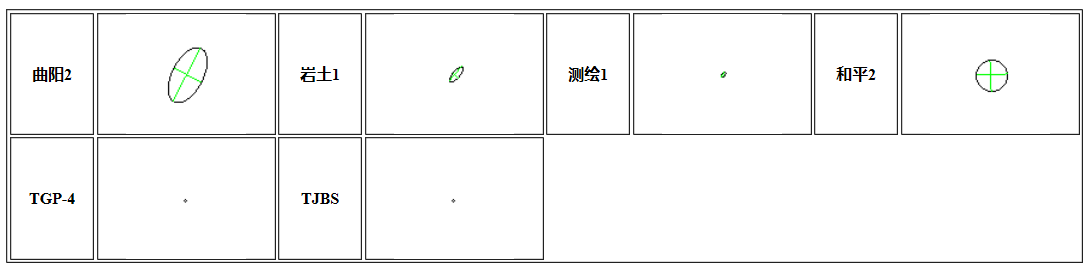
\includegraphics[scale = 0.5]{cgo6.png}
% \end{figure}


\subsection{\Large 二维约束平差}

\begin{center}
    \begin{longtable}{|c|c|c|c|c|}
        \caption{二维当地坐标} \\ \hline
        点ID   & X & X误差 & Y & Y误差 \\ \hline
        曲阳2   & 6061.603222  & 0.013303  & 1410.459802  & 0.010838  \\ \hline
        岩土1   & 5807.168281  & 0.003993  & 2566.110669  & 0.003763  \\ \hline
        测绘1   & 5478.709839  & 0.001541  & 2924.483460  & 0.001413  \\ \hline
        和平2   & 4308.096989  & 0.007423  & 2696.393513  & 0.008690  \\ \hline
        TGP-4 & 5703.239000  & 0.000000  & 2623.323000  & 0.000000  \\ \hline
        TJBS  & 5391.880000  & 0.000000  & 3091.410000  & 0.000000  \\ \hline
        \end{longtable}

        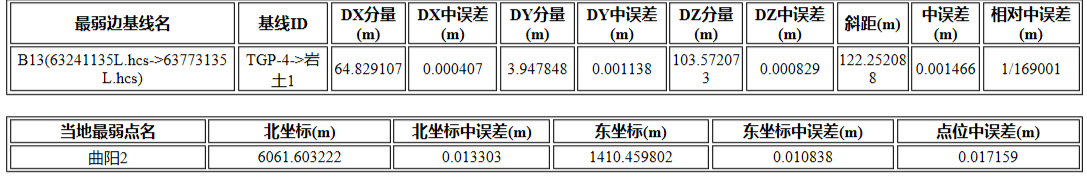
\includegraphics[scale = 0.55]{cgo7.png}
        最弱边最弱点统计

        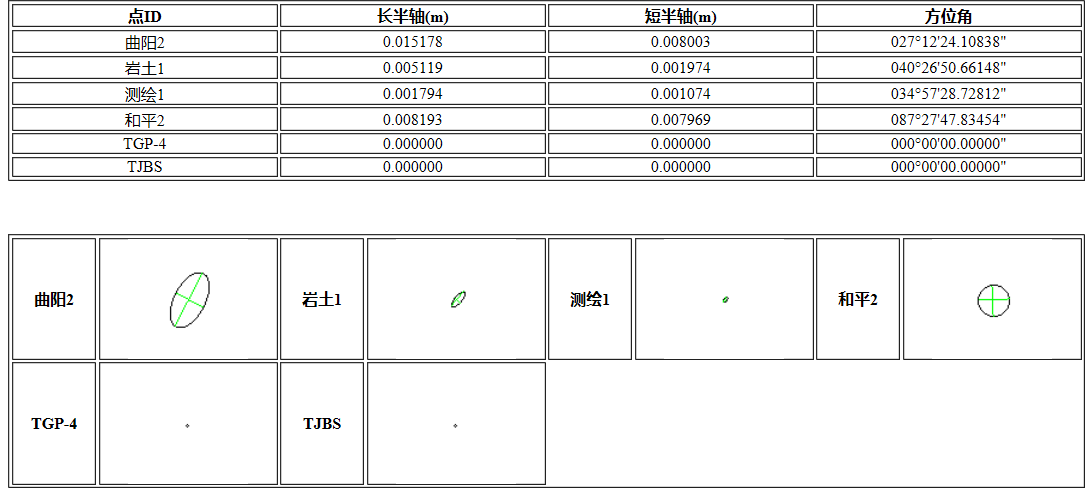
\includegraphics[scale = 0.55]{cgo8.png}
        误差椭圆统计
\end{center}


\subsection{\Large 高程拟合}

\begin{center}
    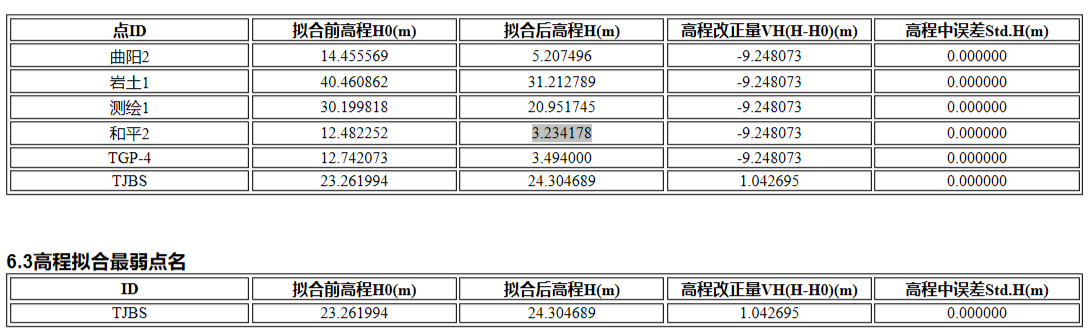
\includegraphics[scale = 0.55]{cgo9.png}
    高程拟合坐标
\end{center}

\newpage
\section{\LARGE 平面控制测量}

\subsection{概述}
该实验通过GPS测量得到的控制点坐标,对感兴趣建筑进行前方交会,计算其三维坐标。

\begin{center}
    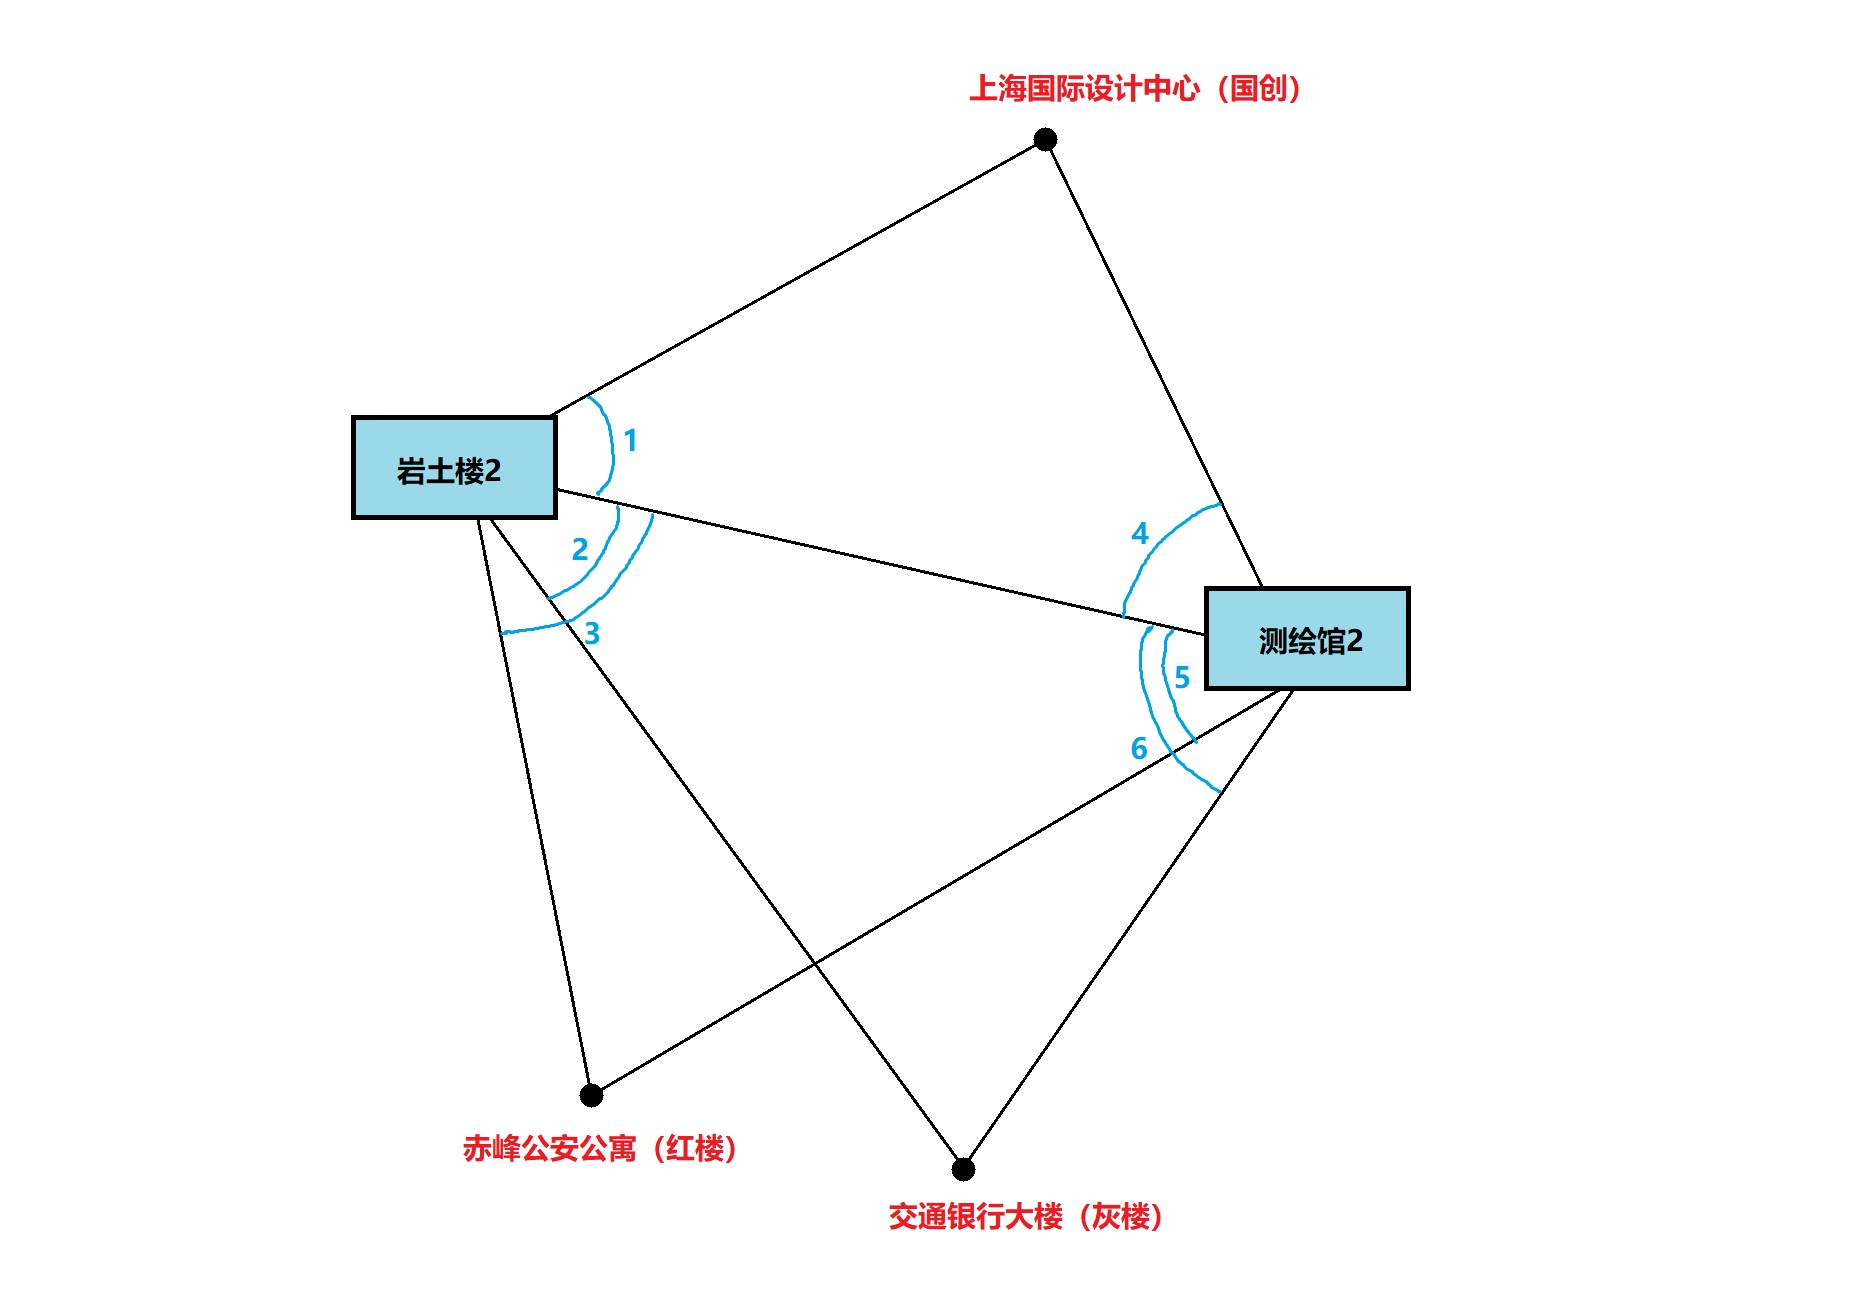
\includegraphics[scale =0.4]{jiaohui.jpg}
    
    交会示意图
\end{center}
如图所示,分别对赤峰公安公寓的避雷针,交通银行大楼的避雷针和上海国际设计中心的东南房屋角点进行了观测。

\subsection{限差要求}

对于水平角的限差要求:
\begin{center}
    \begin{enumerate}
        \item  光学测微器两次重合读数的差对于J1仪器不得超过1秒,对J2型仪器不超过3秒
        \item 半测回归零差的限差对两类仪器各为6秒和8秒
        \item 一测回内2c的互差两类仪器各允许在9秒和13秒以内
        \item 归零后同一方向各测回互差相应地分别为6秒和9秒
    \end{enumerate}
\end{center}

与其注意事项:
\begin{center}
    \begin{enumerate}
        \item  使用照准部微动螺旋和测微螺旋时,其最后旋转方向均应为旋进。
        \item 转动仪器要平稳、匀称,照准目标时,按规定方向旋转,如转过了头,应循此多旋转一圈。
        \item 用望远镜纵丝精确照准目标时,应将目标置于水平丝附近,照准方向目标时在同样的位置。
        \item 原始记录秒值不得更改,错了重测。度、分值若确属读错、记错,须当即在现场改正,此时应将错字整齐划去,在其上填写正确数字。
        \item 在记录观测数据的同时,进行有关部分的计算,仔细检查是否符合限差要求,如有超限,按要求进行重测。
        \item 当照准目标的垂直角超过 时,该方向的2c互差可按同一观测时间段内的相邻测回进行比较,并应在手薄中注明。
    \end{enumerate}
\end{center}

对于垂直角:
\begin{center}
    \begin{enumerate}
        \item  垂直度盘测微器两次读数的差,对于J2型仪器不得超过3″,对于J1型仪器不得超过1″
        \item 垂直角互差(同一方向,由各测回各丝所测得的全部垂直角较差)不得大于10″
        \item 指标差互差(按同方向各测回同一根水平丝所计算的结果的较差)不得大于15″
    \end{enumerate}
\end{center}


\subsection{已知数据与测量成果}

在本报告中仅展示最终结果,记录表格可参照附录

\begin{center}
    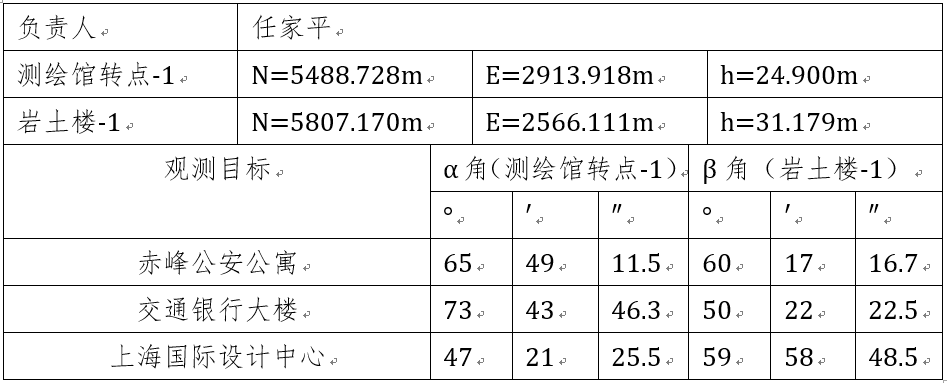
\includegraphics[scale = 0.6]{uvpyjc.png}
    水平角测量结果

    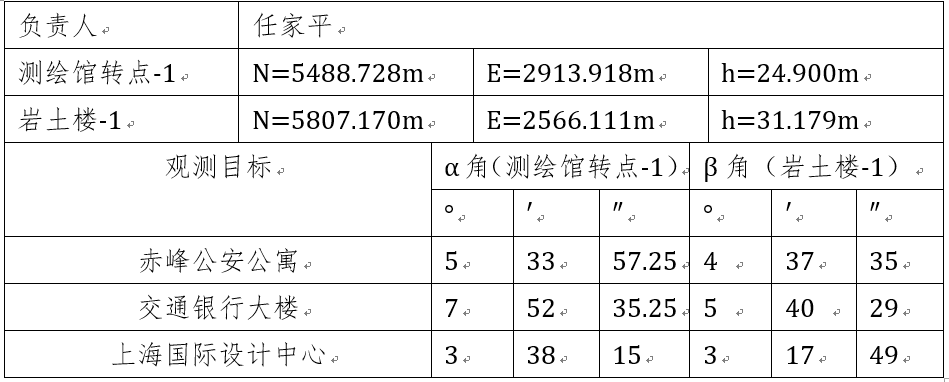
\includegraphics[scale = 0.6]{ivvijc.png}
    垂直角测量结果

\end{center}

\subsection{计算结果}
使用软件 工程测量大师 进行前方交会的XY坐标的计算

\begin{center}
    

    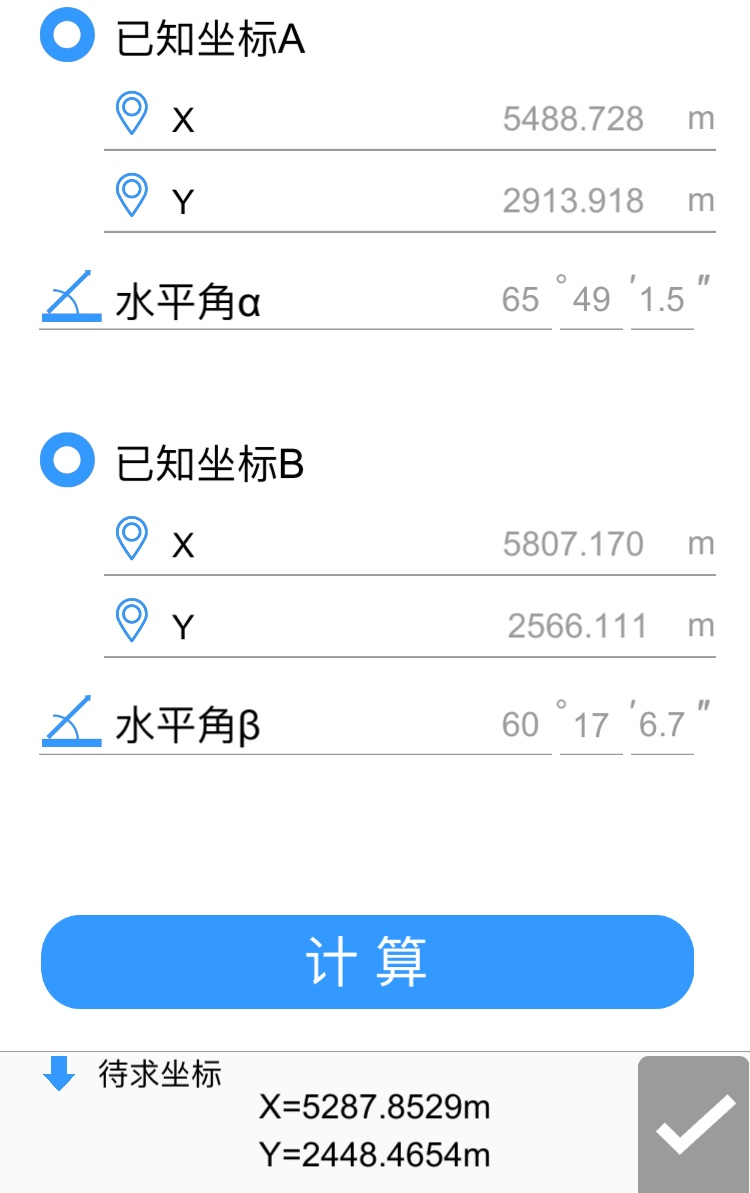
\includegraphics[scale = 0.45]{iifg.jpg}

    赤峰公安公寓天线XY坐标
    
    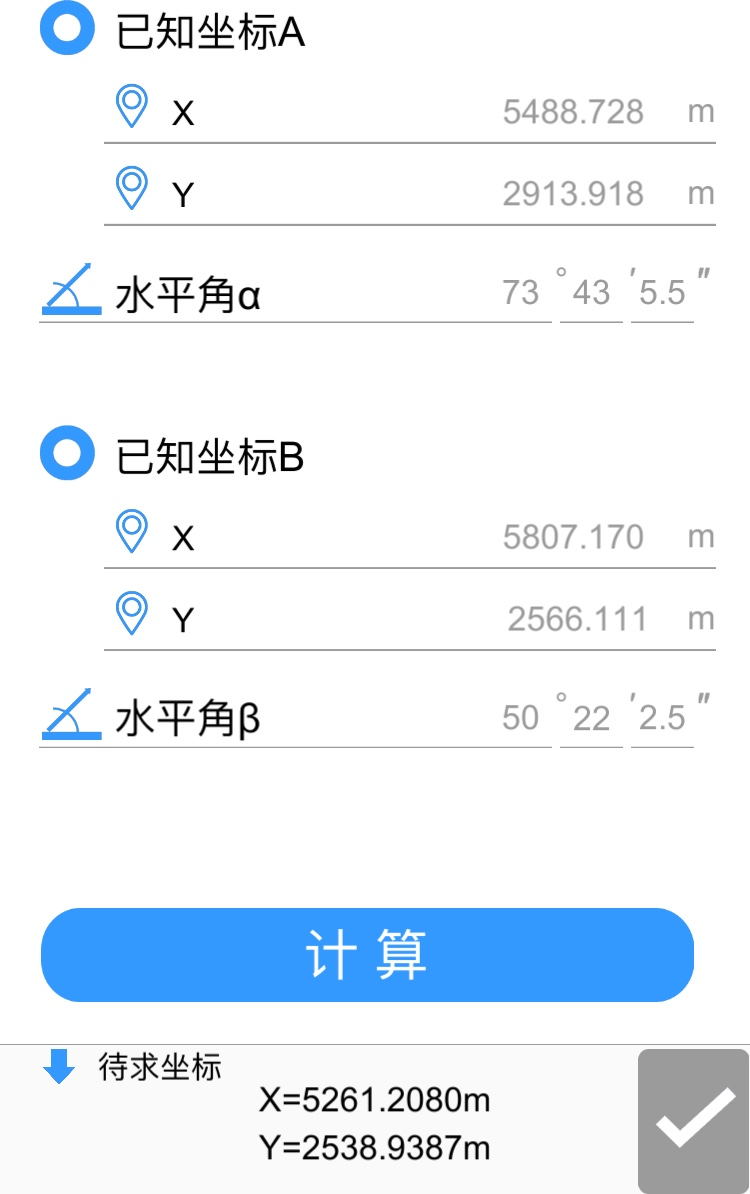
\includegraphics[scale = 0.45]{jcts.jpg}
    
    交通银行大楼天线XY坐标
    
    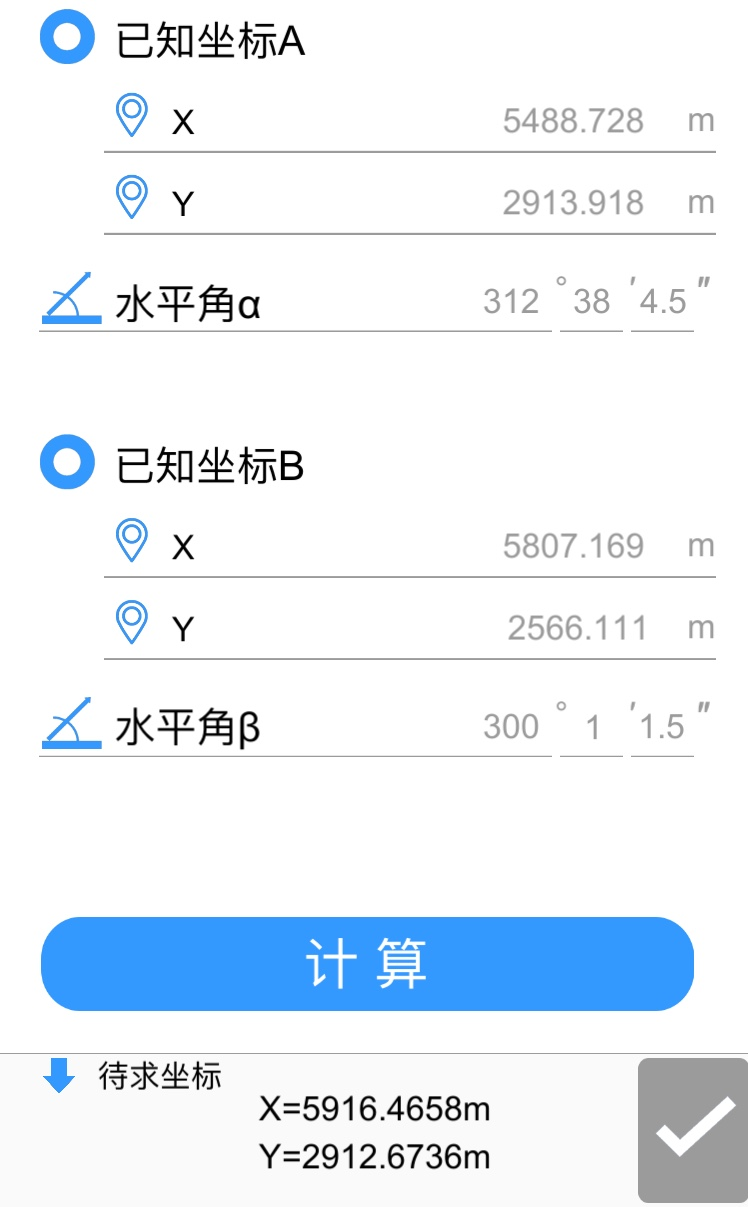
\includegraphics[scale = 0.45]{uhue.jpg}
    
    上海国际设计中心东南角点XY坐标
\end{center}

之后根据几何关系,计算Z坐标,具体公式为:

\begin{center}
    $H_{t} = H_{s} + dis \times tan(\alpha) + h_{s} $
\end{center}
其中 $H_{t}$ 表示目标高,$dis$ 代表测站与观测点平面距离,$h_{s}$表示仪器高,由此可以计算各个待测点的Z坐标。结果如下表所示:

\begin{longtable}{|c|c|c|c|}
    \caption{目标XYZ} \\ \hline
    待测目标点 & X & Y & Z \\ \hline
    赤峰公安公寓 & 5287.861 & 2448.489 & 75.793 \\ \hline
    交通银行大楼 & 5261.141 & 2538.930 & 87.018 \\ \hline
    上海国际设计中心 & 5216.483 & 2912.681 & 53.590\\ \hline
\end{longtable}

\newpage
\section{\LARGE 实习感想}

很荣幸能和其余五位同学组队共同完成本次大地测量实习。暑假俗事缠身,不得不在学期内将实习完成,真是辛苦陈老师了。

所幸实习过程一切都还算顺利,要测量的时候,大家都会在群里打好招呼,第二天大概5:40起床,什么时候有课,那就测到什么时候结束,所以从开始外业的几周里面,还是比较辛苦,深深体会到测量的艰辛。尽管相比大二暑假实习使用的水准仪,这次使用的精密水准仪,解放了双眼,但是一条2.5km长的水准路线反反复复测量4次,还是异常疲惫。

头一次玩GPS接收机,大家骑着自行车,包里塞着鸡哥接收机,脚架套在胸前,骑着破破烂烂的摩拜就前往了目的地公园。周末的太阳甚是毒辣,一天结束后,手臂脖子硬生生的发红,微微胀痛。才明白自己晒伤了,如果现在5月天都是如此,那暑假真是不堪其忧。曲阳公园算是一个微型公园,和平公园倒是挺大。人来人往,总有调皮的小孩子去摸仪器,让人胆战心惊。倒是发现,越是对路边摆放仪器感兴趣的人,他们对测量工作了解的程度越是少。反倒是从事该方面工作的路人,一眼看出了GPS接收机,唯恐避之不及。

在小组的测量过程中,自己在水准测量了北门到西南门高程待测点的第二次往返。由于GPS测量没有注意岩土楼和测绘馆的通视,所以本来一个早上可以测完的前方交会,由于不通视,不知不觉测了两个早上,第一个早上还特别冷,我穿的是短袖短裤,从测绘馆下来,已经没有什么知觉了。

应对这个问题的解决措施是支过去。然而唯一的缺点是GPS的点位误差在短距离测量中,会对测量的精度大打折扣。所幸大家交会结果算出来也能合的上来。

比较煎熬的是写报告,第一次写打报告用 Latex,中途经历重重磨难,所幸在截止日期之前完成了报告,还是比较开心,同时对Latex的使用更加熟练了一些。Latex真是一个神奇的排版工具,能在几天,甚至几小时内生成很多具有书籍质量的印刷品。对于生成复杂表格和数学公式,这一点表现得尤为突出。因此它非常适用于生成高印刷质量的科技和数学类文档。此次实习报告中的很多表格都是直接用Latex的语句直接生成,非常便捷。插入图片可以用数字来控制缩放比例也是比较方便。

本次测量实习真是受益匪浅。




\end{document}